\documentclass[aspectratio=169]{beamer}

\usepackage{../theme}
\usepackage{../boxes}

\title{\textbf{\Huge Krypto Währungen}}
\author{\textcolor{secondarycolor}{\textbf{Christian Laussmann}}}
\date{}

\begin{document}

\frame{\titlepage}





\section{Einführung}


\begin{frame}{Bargeldzahlung}
    \begin{center}
        \begin{tabular}{ccccc}
            
\includegraphics[width=2.5cm]{../icons/Alan} & {\Huge$\longrightarrow$} & 
\includegraphics[width=2cm]{../icons/Coin} & {\Huge$\longrightarrow$} & 
\includegraphics[width=2.5cm]{../icons/Linus}\\
            Alan & & & & Linus\\
        \end{tabular}
    \end{center}
    \vspace{0.5cm}

    \pause
    \textbf{Das funktioniert, weil:}
    \begin{itemize}
        \item Alan \textbf{besitzt} die Münze und \textbf{darf} sie abgeben.
        \item Linus \textbf{besitzt} anschließend die Münze und kann damit bezahlen.
        \item Alan kann Linus die Münze nicht \textbf{wegnehmen} oder die Münze \textbf{erneut ausgeben}.
    \end{itemize}
\end{frame}



\begin{frame}{Überweisung}
    \begin{center}
        \begin{tabular}{ccccc}
            
\includegraphics[width=2cm]{../icons/Alan}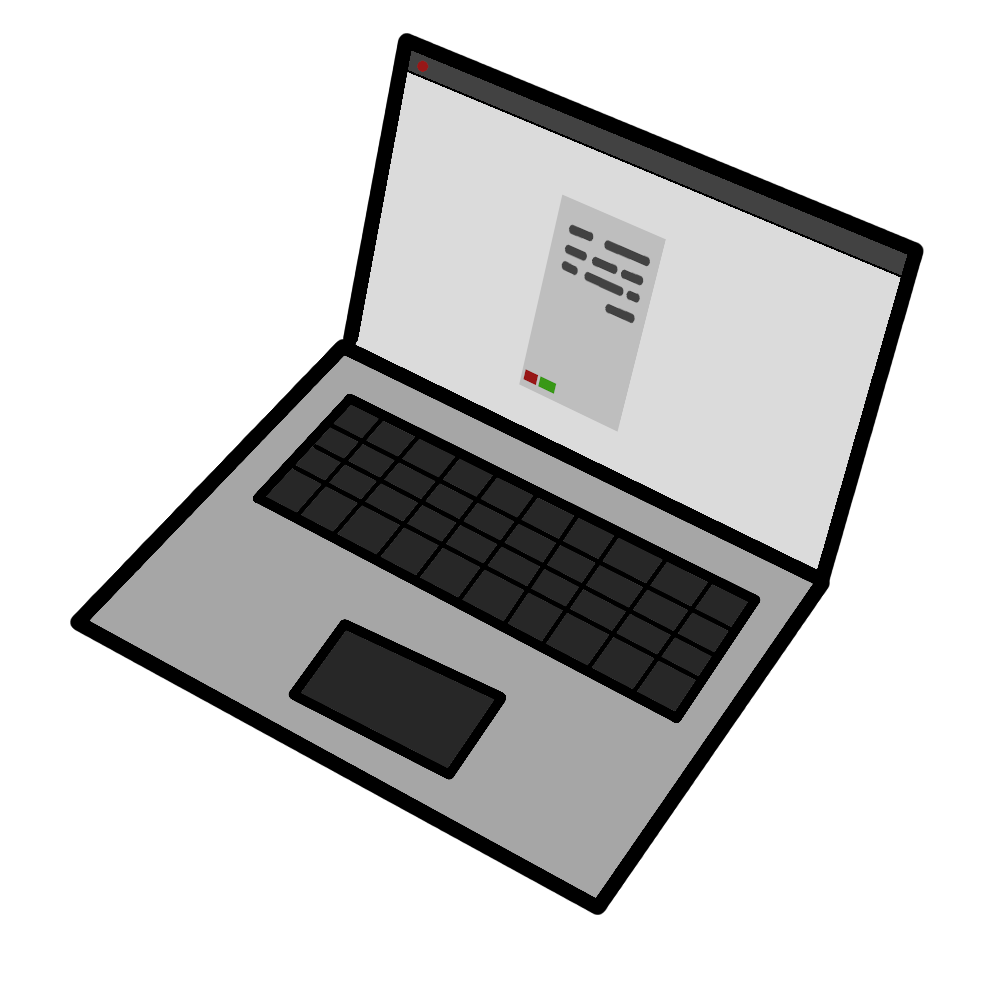
\includegraphics[width=1.5cm]{../icons/ComputerLeft} & {\Huge$\longrightarrow$} & 
\includegraphics[width=2.5cm]{../icons/Bank} & {\Huge$\longrightarrow$} & 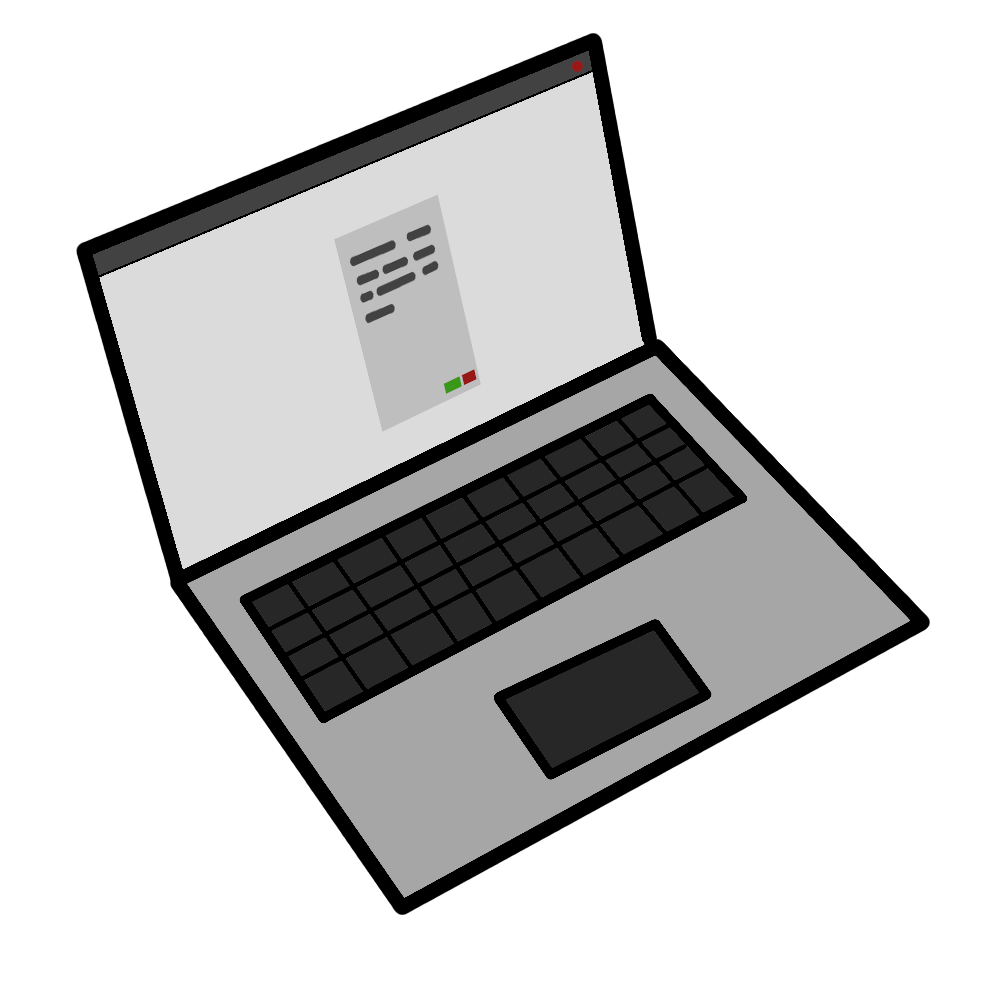
\includegraphics[width=1.5cm]{../icons/ComputerRight}
\includegraphics[width=2cm]{../icons/Linus}\\
            Alan & & Prüfung durch Bank & & Linus\\
        \end{tabular}
    \end{center}
    \vspace{0.5cm}

    \pause
    \begin{itemize}
        \item \textbf{Gültigkeit:} Alans Bank prüft Alans Kontostand. Gesetze und Zentralbanken verhindern Betrug zwischen den Banken.
        \item \textbf{Authorisierung:} Alan hat Zugangsdaten zum Onlinebanking.
        \item \textbf{Unveränderlichkeit:} Sichergestellt durch Gesetze und Zentralbanken.
    \end{itemize}
\end{frame}



\begin{frame}{Krypto-Überweisung}
    \begin{center}
        \begin{tabular}{ccccc}
            
\includegraphics[width=2cm]{../icons/Alan}\hspace*{-0.5cm}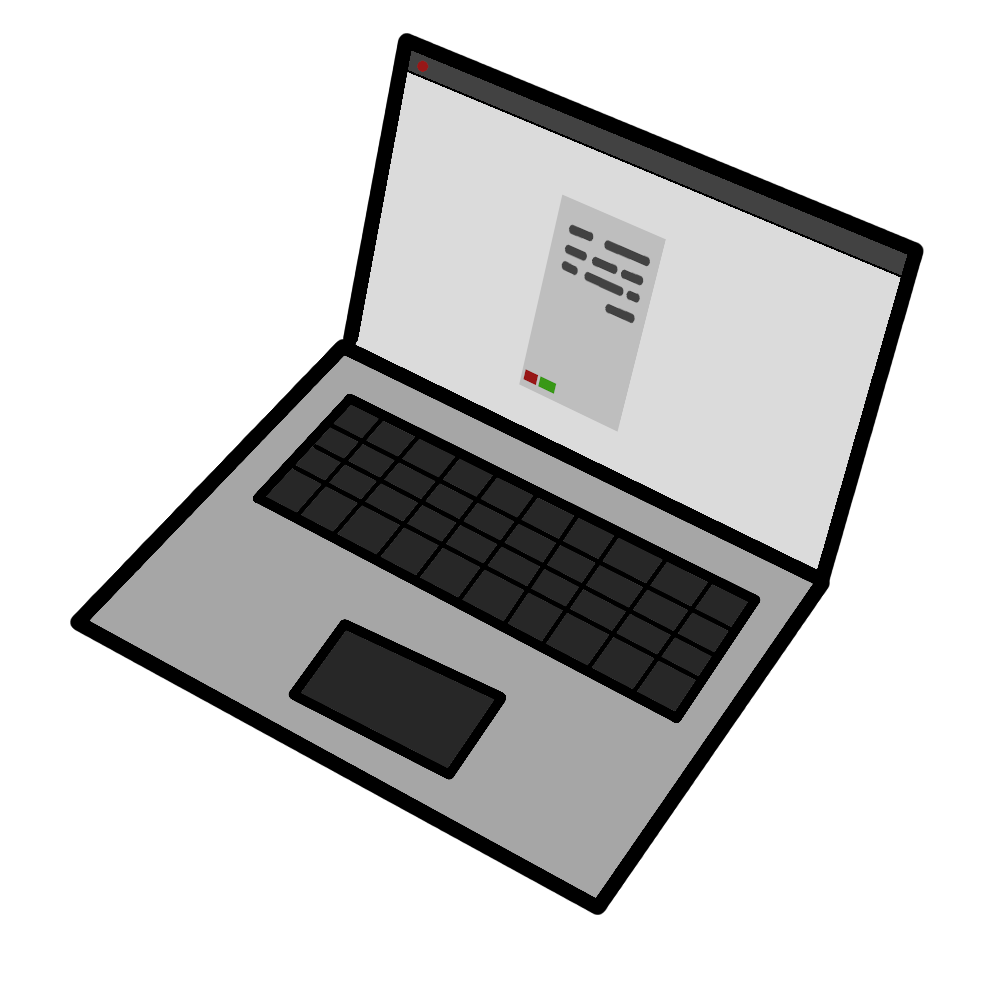
\includegraphics[width=1.5cm]{../icons/ComputerLeft} & {\Huge$\longrightarrow$} & 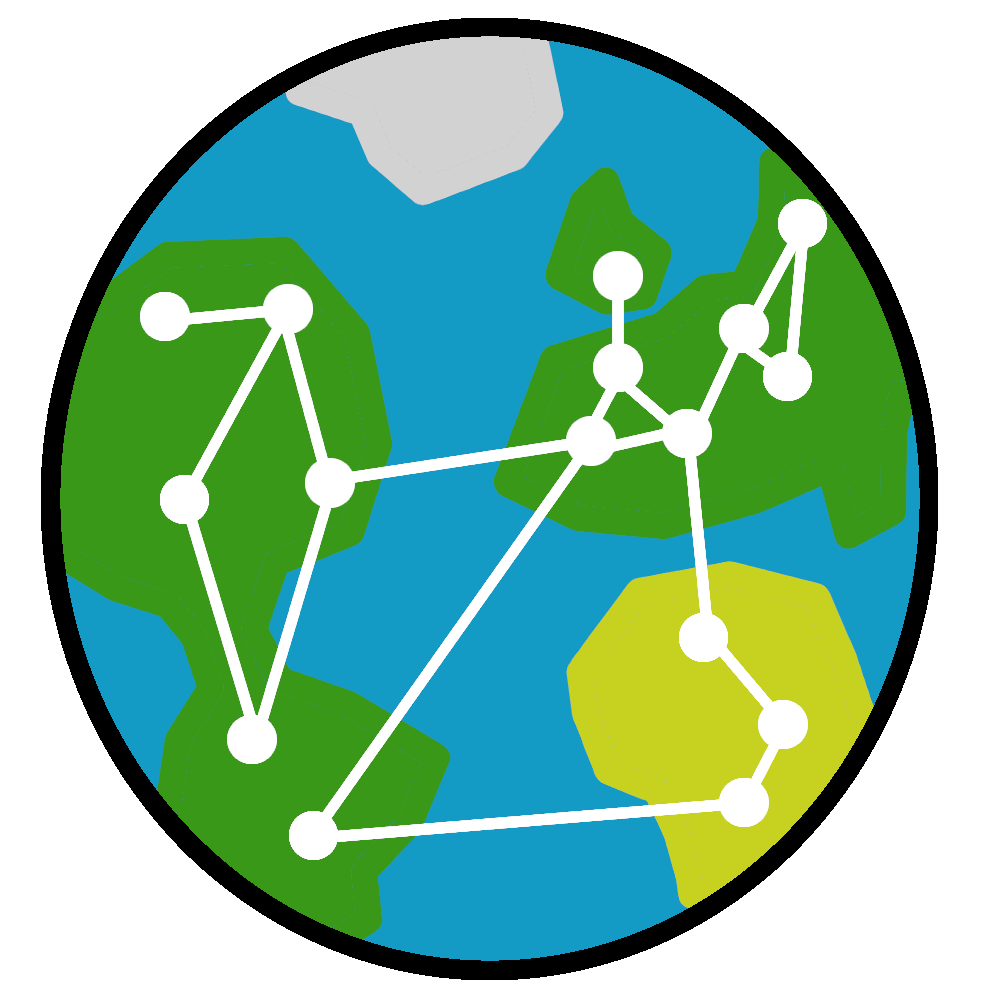
\includegraphics[width=2.5cm]{../icons/Internet}\hspace*{-1.5cm}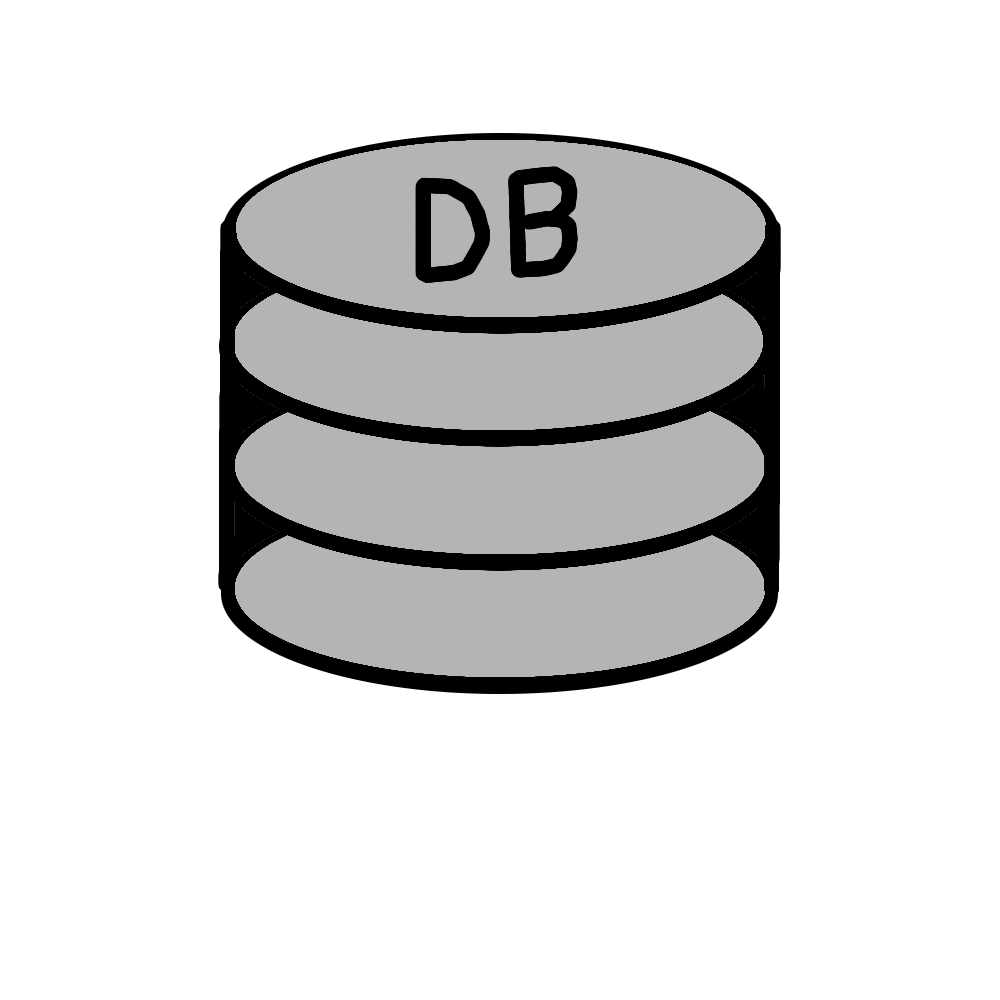
\includegraphics[width=2cm]{../icons/DB} & {\Huge$\longrightarrow$} & 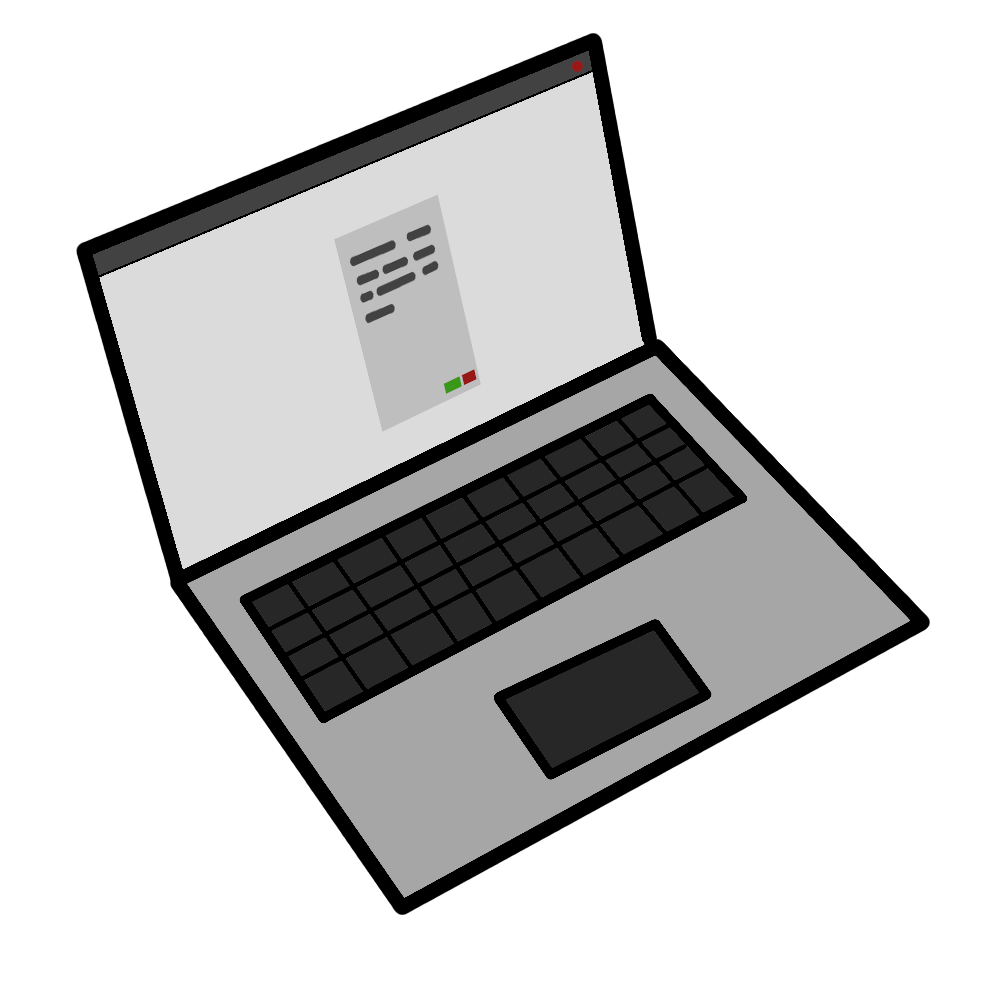
\includegraphics[width=1.5cm]{../icons/ComputerRight}\hspace*{-0.5cm}
\includegraphics[width=2cm]{../icons/Linus}\\
            Alan & & ``Alan sendet Linus 
\includegraphics[width=0.5cm]{../icons/Coin}'' & & Linus\\
        \end{tabular}
    \end{center}
    \vspace{0.5cm}

    \pause
    \begin{itemize}
        \item \textbf{Gültigkeit:} Wer prüft, ob Alan genug Geld hat?
        \item \textbf{Authorisierung:} Wie ist garantiert, dass jeder nur eigenes Geld überweisen kann?
        \item \textbf{Unveränderlichkeit:} Wer garantiert, dass Transaktionen nicht bearbeitet werden?
        \item \textbf{Niemand vertraut den anderen -- nur der Mathematik.}
    \end{itemize}
\end{frame}


\section{Unveränderlichkeit}
\includesectiontitle

\begin{frame}[fragile]{Die Blockchain}
    \begin{center}
        \boxwithtitle{3.85cm}{a}{Block \#1}{
            Transaktion 1\\
            Transaktion 2\\
            ...
        }
        \hspace{0.7cm}
        \boxwithtitle{3.85cm}{b}{Block \#2}{
            Transaktion 3\\
            Transaktion 4\\
            ...
        }
        \hspace{0.7cm}
        \boxwithtitle{3.85cm}{c}{Block \#3}{
            Transaktion 7\\
            Transaktion 8\\
            ...
        }
    \end{center}
    \begin{tikzpicture}[overlay, remember picture]
        \draw[->, line width=2pt] (b) -- (a);
        \draw[->, line width=2pt] (c) -- (b);
    \end{tikzpicture}
\end{frame}


\begin{frame}{Hash-Pointer}
    \begin{center}
        \boxwithtitle{3.85cm}{a}{c6cc}{
            Vorgänger: null\\
            Transaktionen:\\
            ...
        }
        \hspace{0.7cm}
        \boxwithtitle{3.85cm}{b}{afaa}{
            Vorgänger: \textbf{c6cc}\\
            Transaktionen:\\
            ...
        }
        \hspace{0.7cm}
        \boxwithtitle{3.85cm}{c}{7ffa}{
            Vorgänger: \textbf{afaa}\\
            Transaktionen:\\
            ...
        }
    \end{center}
    \begin{tikzpicture}[overlay, remember picture]
        \draw[->, line width=2pt] (b) -- (a);
        \draw[->, line width=2pt] (c) -- (b);
    \end{tikzpicture}
    \pause

    \terminalbox{christian@dev \$\_}{
        \$\_\;\; echo 'Hallo Christian' | sha256sum\\
        \phantom{...} 37c24999d0c3f6b0d295c19699bc121c6b7c194fb957b15bdb3582c60edf3a1f\\~\\
        \$\_\;\; echo 'hallo christian' | sha256sum\\
        \phantom{...} e52c859ed0b18b5dcce6d177caf000b19c7c578504f9dbc626580387b1f79ab5
    }
\end{frame}


\begin{frame}{Gebrochene Kette}
    \begin{center}
        \boxwithtitle{3.85cm}{a}{c6cc}{
            Vorgänger: null\\
            Transaktionen:\\
            ...
        }
        \hspace{0.7cm}
        \boxwithtitle{3.85cm}{b}{\textcolor{myviolet}{afaa}}{
            Vorgänger: \textbf{c6cc}\\
            Transaktionen:\\
            \textcolor{myviolet}{\textbf{Alan sendet 4}}
        }
        \hspace{0.7cm}
        \boxwithtitle{3.85cm}{c}{7ffa}{
            Vorgänger: \textbf{\textcolor{myviolet}{afaa}}\\
            Transaktionen:\\
            ...
        }
    \end{center}
    \begin{tikzpicture}[overlay, remember picture]
        \draw[->, line width=2pt] (b) -- (a);
        \draw[->, line width=2pt] (c) -- (b);
    \end{tikzpicture}

    \pause
    \begin{center}
        \boxwithtitle{3.85cm}{e}{c6cc}{
            Vorgänger: null\\
            Transaktionen:\\
            ...
        }
        \hspace{0.7cm}
        \boxwithtitle{3.85cm}{f}{\textcolor{myblue}{6ae7}}{
            Vorgänger: \textbf{c6cc}\\
            Transaktionen:\\
            \textcolor{myblue}{\textbf{Alan sendet 1}}
        }
        \hspace{0.7cm}
        \boxwithtitle{3.85cm}{g}{7ffa}{
            Vorgänger: \textbf{\textcolor{myviolet}{afaa}}\\
            Transaktionen:\\
            ...
        }
    \end{center}
    \begin{tikzpicture}[overlay, remember picture]
        \draw[->, line width=2pt] (f) -- (e);
        \draw[->, dashed, line width=2pt, color=myred] (g) -- (f);
    \end{tikzpicture}
\end{frame}


\begin{frame}{Reparatur einer gebrochenen Kette}
    \begin{center}
        \boxwithtitle{3.85cm}{a}{c6cc}{
            Vorgänger: null\\
            Transaktionen:\\
            ...
        }
        \hspace{0.7cm}
        \boxwithtitle{3.85cm}{b}{\textcolor{myblue}{6ae7}}{
            Vorgänger: \textbf{c6cc}\\
            Transaktionen:\\
            \textcolor{myblue}{\textbf{Alan sendet 1}}
        }
        \hspace{0.7cm}
        \boxwithtitle{3.85cm}{c}{7ffa}{
            Vorgänger: \textbf{\textcolor{myviolet}{afaa}}\\
            Transaktionen:\\
            ...
        }

        \vspace{1.5cm}

        \boxwithtitle{3.85cm}{e}{22ea}{
            Vorgänger: \textbf{5aff}\\
            Transaktionen:\\
            ...
        }
        \hspace{0.7cm}
        \boxwithtitle{3.85cm}{d}{5aff}{
            Vorgänger: \textbf{7ffa}\\
            Transaktionen:\\
            ...
        }
    \end{center}
    \begin{tikzpicture}[overlay, remember picture]
        \draw[->, line width=2pt] (b) -- (a);
        \draw[->, dashed, line width=2pt, color=myred] (c) -- (b);
        \draw[->, line width=2pt] (d) -- (c);
        \draw[->, line width=2pt] (e) -- (d);
    \end{tikzpicture}
\end{frame}

\begin{frame}{Reparatur einer gebrochenen Kette}
    \begin{center}
        \boxwithtitle{3.85cm}{a}{c6cc}{
            Vorgänger: null\\
            Transaktionen:\\
            ...
        }
        \hspace{0.7cm}
        \boxwithtitle{3.85cm}{b}{\textcolor{myblue}{6ae7}}{
            Vorgänger: \textbf{c6cc}\\
            Transaktionen:\\
            \textcolor{myblue}{\textbf{Alan sendet 1}}
        }
        \hspace{0.7cm}
        \boxwithtitle{3.85cm}{c}{\textcolor{myblue}{dad4}}{
            Vorgänger: \textbf{\textcolor{myblue}{6ae7}}\\
            Transaktionen:\\
            ...
        }

        \vspace{1.5cm}

        \boxwithtitle{3.85cm}{e}{22ea}{
            Vorgänger: \textbf{5aff}\\
            Transaktionen:\\
            ...
        }
        \hspace{0.7cm}
        \boxwithtitle{3.85cm}{d}{5aff}{
            Vorgänger: \textbf{\textcolor{myviolet}{7ffa}}\\
            Transaktionen:\\
            ...
        }
    \end{center}
    \begin{tikzpicture}[overlay, remember picture]
        \draw[->, line width=2pt] (b) -- (a);
        \draw[->, line width=2pt] (c) -- (b);
        \draw[->, dashed, line width=2pt, color=myred] (d) -- (c);
        \draw[->, line width=2pt] (e) -- (d);
    \end{tikzpicture}
\end{frame}

\begin{frame}{Reparatur einer gebrochenen Kette}
    \begin{center}
        \boxwithtitle{3.85cm}{a}{c6cc}{
            Vorgänger: null\\
            Transaktionen:\\
            ...
        }
        \hspace{0.7cm}
        \boxwithtitle{3.85cm}{b}{\textcolor{myblue}{6ae7}}{
            Vorgänger: \textbf{c6cc}\\
            Transaktionen:\\
            \textcolor{myblue}{\textbf{Alan sendet 1}}
        }
        \hspace{0.7cm}
        \boxwithtitle{3.85cm}{c}{\textcolor{myblue}{dad4}}{
            Vorgänger: \textbf{\textcolor{myblue}{6ae7}}\\
            Transaktionen:\\
            ...
        }

        \vspace{1.5cm}

        \boxwithtitle{3.85cm}{e}{22ea}{
            Vorgänger: \textbf{\textcolor{myviolet}{5aff}}\\
            Transaktionen:\\
            ...
        }
        \hspace{0.7cm}
        \boxwithtitle{3.85cm}{d}{\textcolor{myblue}{85a7}}{
            Vorgänger: \textbf{\textcolor{myblue}{dad4}}\\
            Transaktionen:\\
            ...
        }
    \end{center}
    \begin{tikzpicture}[overlay, remember picture]
        \draw[->, line width=2pt] (b) -- (a);
        \draw[->, line width=2pt] (c) -- (b);
        \draw[->, line width=2pt] (d) -- (c);
        \draw[->, dashed, line width=2pt, color=myred] (e) -- (d);
    \end{tikzpicture}
\end{frame}

\begin{frame}{Nonce und Hash-Challenge}
    \begin{center}
        \boxwithtitle{3.85cm}{a}{00a4}{
            Nonce: 42\\
            Vorgänger: null\\
            Transaktionen:\\
            ...
        }
        \hspace{0.7cm}
        \boxwithtitle{3.85cm}{b}{002e}{
            Nonce: 7736\\
            Vorgänger: \textbf{00a4}\\
            Transaktionen:\\
            ...
        }
        \hspace{0.7cm}
        \boxwithtitle{3.85cm}{c}{00fa}{
            Nonce: 4322\\
            Vorgänger: \textbf{002e}\\
            Transaktionen:\\
            ...
        }
    \end{center}
    \begin{tikzpicture}[overlay, remember picture]
        \draw[->, line width=2pt] (b) -- (a);
        \draw[->, line width=2pt] (c) -- (b);
    \end{tikzpicture}
    \begin{itemize}
        \item Wir akzeptieren nur Hash-Werte mit mindestens $X$ Nullen
        \item Passende Nonce durch ausprobieren finden \textbf{(\emph{Mining})}
    \end{itemize}
\end{frame}

\begin{frame}{Hash-Challenge}
    \terminalbox{christian@dev \$\_}{
        \$\_\;\; echo '\textbf{Alan sendet 3. \textcolor{myblue}{Nonce: 737}. Vorgänger: 00af}' | sha256sum\\
        \phantom{...} \textcolor{myviolet}{96c7...}\\~\\\pause
        \$\_\;\; echo '\textbf{Alan sendet 3. \textcolor{myblue}{Nonce: 325}. Vorgänger: 00af}' | sha256sum\\
        \phantom{...} \textcolor{myviolet}{b95a...}\\~\\\pause
        \$\_\;\; echo '\textbf{Alan sendet 3. \textcolor{myblue}{Nonce: 129}. Vorgänger: 00af}' | sha256sum\\
        \phantom{...} \textcolor{myviolet}{0ad2...}\\~\\\pause
        \$\_\;\; echo '\textbf{Alan sendet 3. \textcolor{myblue}{Nonce: 729}. Vorgänger: 00af}' | sha256sum\\
        \phantom{...} \textcolor{myviolet}{101d...}\\
        ...
    }
\end{frame}

\begin{frame}{Fazit bis hier}
    \begin{center}
        \boxwithtitle{3.85cm}{a}{00a4}{
            Nonce: 43732\\
            Vorgänger: null\\
            Transaktionen:\\
            ...
        }
        \hspace{0.7cm}
        \boxwithtitle{3.85cm}{b}{\textcolor{myred}{af3f}}{
            Nonce: 77236\\
            Vorgänger: \textbf{00a4}\\
            Transaktionen:\\
            \textcolor{myred}{\textbf{Alan sendet 1}}
        }
        \hspace{0.7cm}
        \boxwithtitle{3.85cm}{c}{000a}{
            Nonce: 9776762\\
            Vorgänger: \textbf{\textcolor{myred}{006b}}\\
            Transaktionen:\\
            ...
        }

        \vspace{1cm}

        \boxwithtitle{3.85cm}{e}{009d}{
            Nonce: 42\\
            Vorgänger: \textbf{00e3}\\
            Transaktionen:\\
            ...
        }
        \hspace{0.7cm}
        \boxwithtitle{3.85cm}{d}{00e3}{
            Nonce: 334221\\
            Vorgänger: \textbf{000a}\\
            Transaktionen:\\
            ...
        }
    \end{center}
    \begin{tikzpicture}[overlay, remember picture]
        \draw[->, line width=2pt] (b) -- (a);
        \draw[->, dashed, line width=2pt, color=myred] (c) -- (b);
        \draw[->, line width=2pt] (d) -- (c);
        \draw[->, line width=2pt] (e) -- (d);
    \end{tikzpicture}
\end{frame}





\section{Authorisierung}
\includesectiontitle

\begin{frame}{Accounterstellung}
    Bild: Alan neben Public Key Adresse
    \begin{itemize}
        \item Wallet erzeugt Public- und Private-Key
        \item Public-Key (bzw. Ableitung davon) bildet `Kontonummer'
    \end{itemize}
\end{frame}


\begin{frame}{Überweisung Authorisieren}
    Bild: Alan neben Private Key
    \begin{itemize}
        \item Signatur der Überweisung mittels Private-Key
        \item Signatur kann durch Public-Key von jedem überprüft werden
    \end{itemize}
\end{frame}





\section{Gültigkeit}
\includesectiontitle

\begin{frame}{Wann ist Transaktion gültig?}
    Bild: Block mit grünem Haken
    \begin{itemize}
        \item Transaktion wurde authorisiert $\Rightarrow$ Signatur
        \item Sender hat genug Geld $\Rightarrow$ In vorherigen Blöcken nach unverbrauchter Gutschrift suchen
    \end{itemize}
\end{frame}





\section{Mining}
\includesectiontitle

\begin{frame}{Blöcke erschaffen}
    Bild: Miner hämmert auf Block rum
    \begin{itemize}
        \item Miner haben jeweils Kopie der Blockchain
        \item Miner versuchen jeweils neue Blöcke anzuhängen und allen mitzuteilen
        \item Nur gültige neue Blöcke werden von anderen Minern aufgenommen
    \end{itemize}
\end{frame}


\begin{frame}{Woher kommt das Geld?}
    Bild: Miner hämmert auf Block rum -- Münze daneben
    \begin{itemize}
        \item Miner bekommt Belohnung für neuen Block
        \item Miner werden \textbf{aus Eigennutz das Protokoll einhalten}, da ihr Block sonst nicht akzeptiert wird
    \end{itemize}
\end{frame}


\begin{frame}{Fork}
    Bild: Kette mit Fork
    \begin{itemize}
        \item Mittelfristig gewinnt die längere Kette
    \end{itemize}
\end{frame}






% End and Bonus

%% This file contains the last frame in every presentation

\section{Ende}

\begin{frame}{}
    Foto
    \textbf{Christian Laussmann}\\
    LinkedIn:\\
    GitHub: \href{https://github.com/claussmann}{\textcolor{secondarycolor}{github.com/claussmann}}

    \vspace{1cm}
    Vortragsthemen (Auswahl):
    \begin{itemize}
        \item Blockchains \& Kryptowährungen
        \item Kryptographie, Signaturen und Authentifizierung
        \item Computational Social Choice
        \item IT-Security
        \item Softwareentwicklung \& -Architektur
    \end{itemize}
\end{frame}




\section{Bonus: Quick Facts}


\begin{frame}{Bitcoin ist Anonym}
    Bild: Fragezeichen
    \pause
    Bitcoin adresse Beispiel
\end{frame}


\begin{frame}{Niemand kennt meinen Bitcoin-Kontostand}
    Bild: Fragezeichen
    \pause
    Bild: Miner
\end{frame}


\begin{frame}{Bitcoin ist sicher gegen Quantencomputer}
    Bild: Fragezeichen
\end{frame}

\end{document}
